\chapter{Design}
\label{ch:Design}

Ein wichtiger Teil dieser Arbeit ist die Erstellung eines Datensatzes, welcher zur Klassifikation dienen soll.
Es wird eine Smartphone-App erstellt, welche einen Datensatz eines Studienteilnehmer aufzeichnen und exportieren soll. 
Daraufhin liegen die Daten vor und könnnen in einer Verarbeitungspipeline analysiert, bzw. klassifiziert werden.

Die Studie wurde so konzipiert, Atemaussetzer währrend des Schlafens zu klassifizieren. 
Während der Studie wurde jeder Datensatz im Bett des Teilnehmers aufgezeichnet, um sein Wohlbefinden und somit auch die Qualität der Daten zu erhöhen.
\todo{den satz besser :)}

\section{Studienablauf}
Für die Studie wurde eine Teilnehmeranzahl von 10 Personen gewählt, welche die nötige Vielfältigkeit liefern soll.
Des weiteren wurden pro Teilnehmer ein Datensatz an 3 verschiedene Positionen aufgezeichnet, auf dem Bauch, dem Rücken, sowie auf der Seite liegend.

Eine Fragestellung der Studie war, wie ein Atemaussetzer \glqq simuliert\grqq werden soll. 
Es wurde entschieden, dass die Studie ein zentrales Schlafapnoe erkennen soll. 
Demzufolge soll der Studienteilnehmer in einer vordefinierten Reihenfolge einen Atemaussetzer \glqq simulieren\grqq, indem er die Luft für eine gewisse Zeit anhält.
Um unterschiedliche Längen von Atemaussetzern aufzuzeichnen wurden $10\si{\s}$, $20\si{\s}$ und $30\si{\s}$ gewählt, in denen der Teilnehmer die Luft anhalten soll. 
Nun muss ein geeigneter Ablauf gewählt werden, wodurch sich die Ereignisse nicht überschneiden.
Auf der Suche, wie Lange die Regeneration dauere, nachdem eine Person die Luft angehalten hat, ergab sich durch das Schaubild \ref{fig_respiration_regeneration}, 
dass die Person ca die gleiche Zeit zur Regeneration benötigt, wie sie die Luft zuvor angehalten hat.
Diese Zeit wurde nun zusätlich in der Studie mit eingebracht und daraus ergibt sich folgender Ablauf:
\begin{figure}[ht]
    \centering
    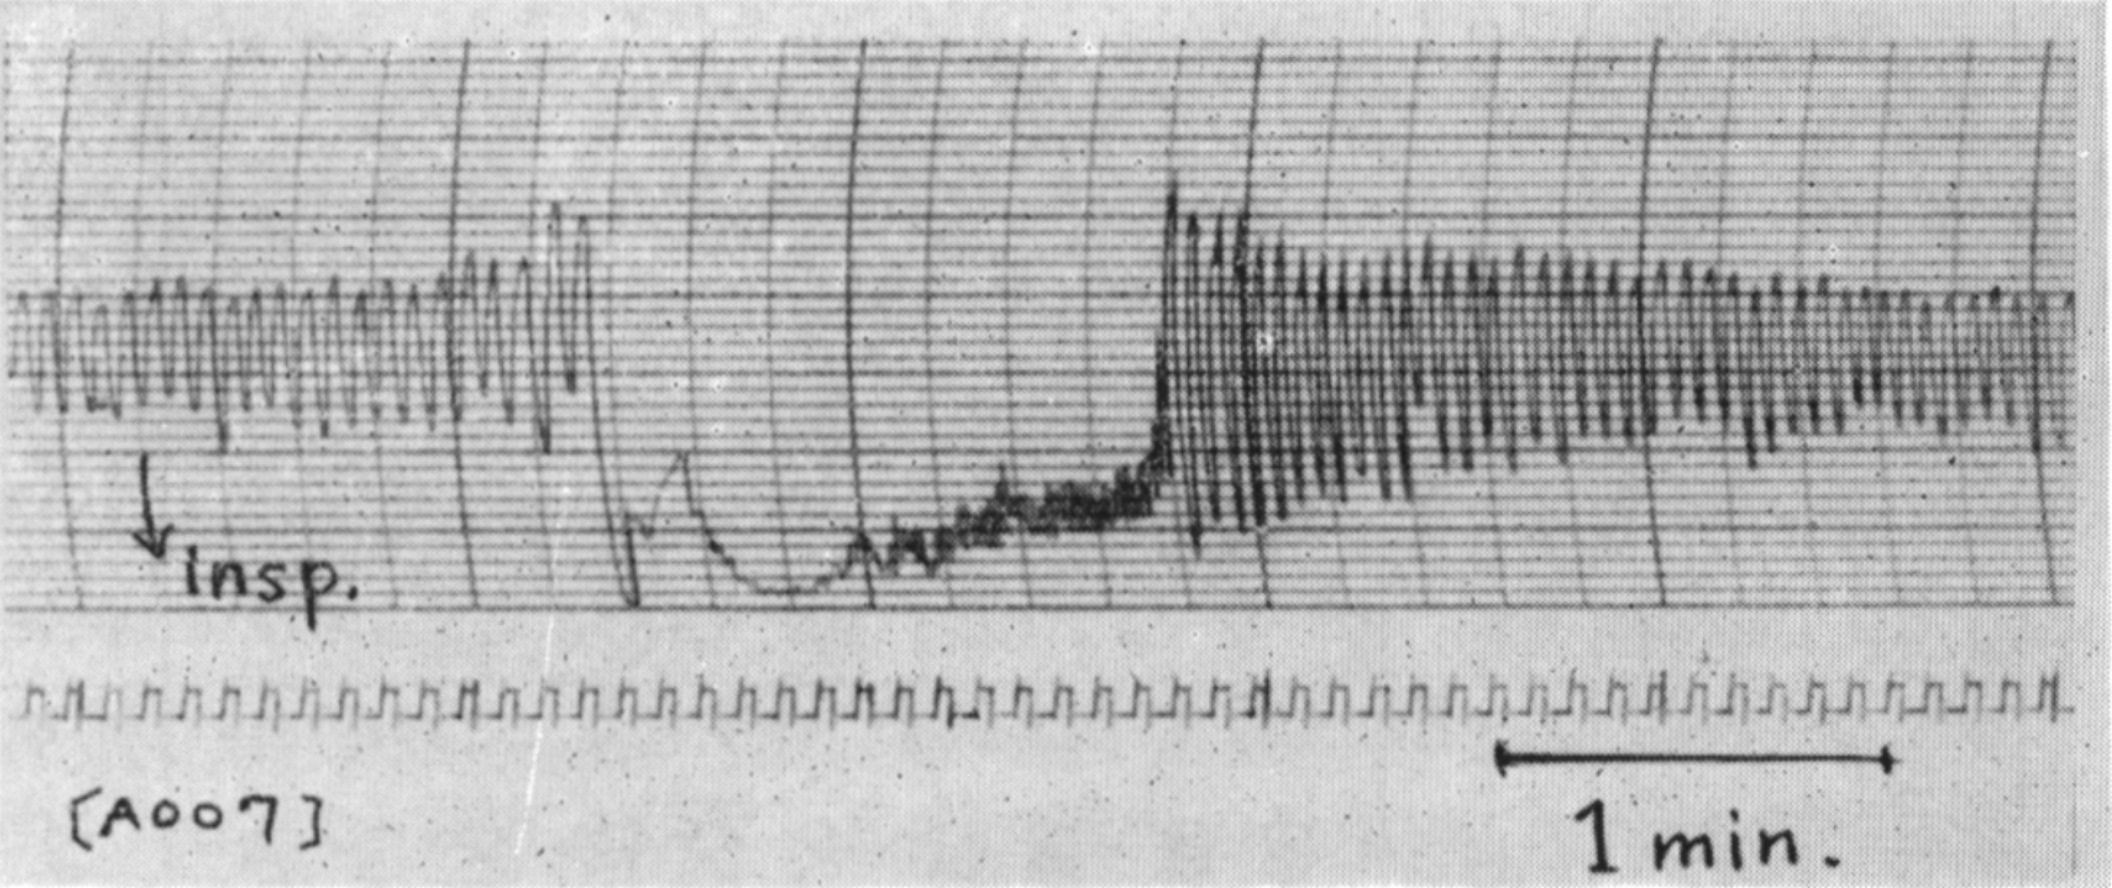
\includegraphics[width=0.66\textwidth]{images/respiration/respiration_regeneration}
    \caption{Regenerationsphase nach Luft anhalten \cite{hernandez_cardiac_nodate}.}
    \label{fig_respiration_regeneration}
\end{figure}

\todo{Füge bild zum Ablauf ein, so dass es nicht nach ner dummen aufzählung aussieht}

Dieser Ablauf wurde nun pro Studienteilnehmer jeweils bei den 3 Positionen durchgeführt.

\todo{Raum beschreiben, dass ich leise war, bzw den raum verlassen habe... ton vorher aufgenommen gibt anweisungen}

wie bekommt der Nutzer anweisungen? alles über Ton
bild mit erklärung, warum die atempausen (regeneration) $https://www.jstage.jst.go.jp/article/jjphysiol1950/17/1/17_1_43/_pdf$

Anweisungen kommen über die App per Ton aus den eSense-Earpods.

\begin{itemize}
    \item wie viele Personen wurden ausgewaehlt
    \item wie ist der ablauf der studie
    \begin{itemize}
        \item was bekommt der Nutzer fuer anweisungen
    \end{itemize}
\end{itemize}
